\documentclass[tikz,border=5pt]{standalone}
\usepackage{libertinust1math}
\usetikzlibrary{calc,arrows.meta}
% https://ask.latexstudio.net/ask/question/17575.html
% https://tex.stackexchange.com/questions/297525/drawing-cyclic-quiver
\begin{document}
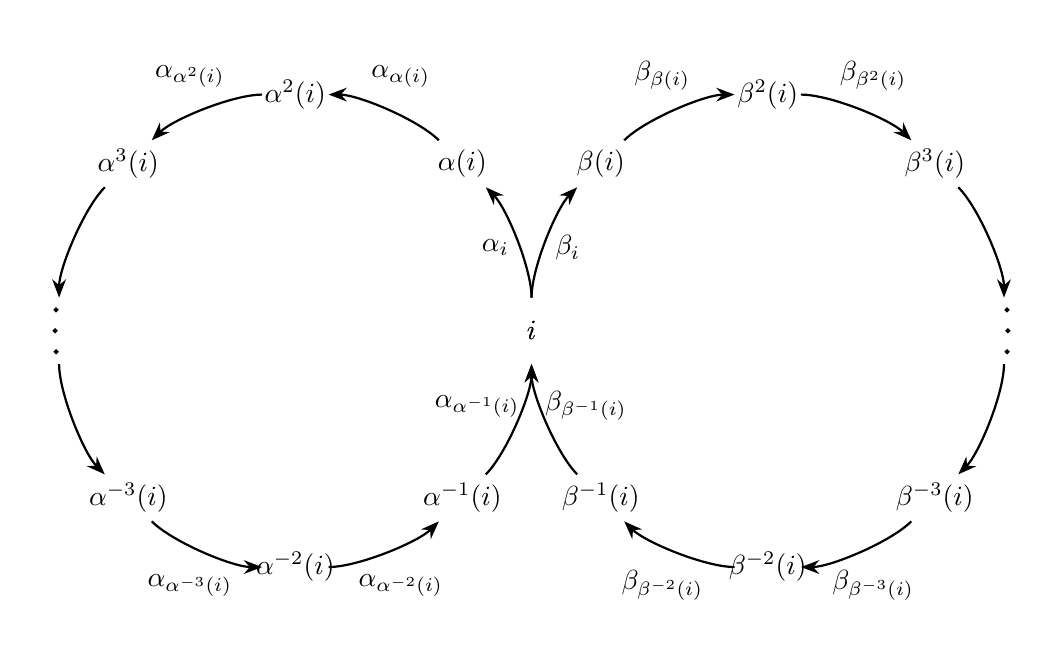
\begin{tikzpicture}
\begin{scope}[xshift=3cm]
\foreach \ang/\content/\radius/\lab in {
    180/{$i$}/2.75/{$\beta_i$},
    135/{$\beta(i)$}/3.5/{$\beta_{\beta(i)}$},
    90/{$\beta^2(i)$}/3.5/{$\beta_{\beta^2(i)}$},
    45/{$\beta^3(i)$}/3.5/{},
    0/{}/3.5/{},
    -45/{$\beta^{-3}(i)$}/3.5/{$\beta_{\beta^{-3}(i)}$},
    -90/{$\beta^{-2}(i)$}/3.5/{$\beta_{\beta^{-2}(i)}$},
    -135/{$\beta^{-1}(i)$}/2.5/{$\beta_{\beta^{-1}(i)}$}%
}{
  \draw[-Stealth,thick,shorten <=12pt, shorten >=12pt] ($(0,0)+(\ang:3)$) node[circle] {\content} arc (\ang:\ang-45:3);
  \node[anchor=center,circle] at ($(0,0)+(\ang-22.5:\radius)$) {\lab};
}
\foreach \ang in {-5,0,5}{\draw[fill=black] ($(0,0)+(\ang:3.05)$) circle (.025);}
\end{scope}
\begin{scope}[xshift=-3cm]
\foreach \ang/\content/\radius/\lab in {
    0/{$i$}/2.75/{$\alpha_i$},
    45/{$\alpha(i)$}/3.5/{$\alpha_{\alpha(i)}$},
    90/{$\alpha^2(i)$}/3.5/{$\alpha_{\alpha^2(i)}$},
    135/{$\alpha^3(i)$}/3.5/{},
    180/{}/3.5/{},
    225/{$\alpha^{-3}(i)$}/3.5/{$\alpha_{\alpha^{-3}(i)}$},
    270/{$\alpha^{-2}(i)$}/3.5/{$\alpha_{\alpha^{-2}(i)}$},
    315/{$\alpha^{-1}(i)$}/2.5/{$\alpha_{\alpha^{-1}(i)}$}%
}{
  \draw[Stealth-,thick,shorten <=12pt, shorten >=12pt] ($(0,0)+(\ang:3)$) node[circle] {\content} arc (\ang:\ang-45:3);
  \node[anchor=center,circle] at ($(0,0)+(\ang+22.5:\radius)$) {\lab};
}
\foreach \ang in {-5,0,5}{\draw[fill=black] ($(0,0)-(\ang:3.05)$) circle (.025);}
\end{scope}
\end{tikzpicture}
\end{document}